
\section{Relatives Vorkommen (Referenz)}
Ein einfacher Ansatz, der als Referenz zum Finden relevanter Wörter eines Tages dient ist der, das Auftreten jedes Tokens im Tageskorpus mit dem Auftreten im Referenzkorpus ins Verhältnis zu setzen.\\
Hierbei werden um eine Vergleichbarkeit zwischen verschiednen Tagen zu gewährleisten die Frequenzen der Wörter über die Anzahl aller Tokens im Tages bzw. Referenzkorpus normiert.\\

	\emph{Formel: } 
	\begin{equation}
	sig_{freqratio}(w) = \frac{\frac{k_{day}}{n_{day}}}{\frac{k_{2014}}{n_{2014}}}
	\end{equation}
	$k_{day}$: Frequenz des Tokens an einem Tag\\
	$n_{day}$: Summe der Frequenzen aller Tokens eines Tages\\
	$k_{2014}$: Frequenz des Tokens im Referenz Zeitrahmen (2014)\\
	$n_{day}$: Summe der Frequenzen aller Tokens im Referenzzeitraum (2014)\\
	

In Abbildung~\ref{pic.rel_freq} stellt die schwarze Gerade dar, wie sich der Wert der relativen Frequenz verhält, wenn die Anzahl des Auftretens eines Tokens variiert. Die senkrechte roten Linien markiert die Anzahl der Tokens, bei denen das relative Auftreten dem relativen Auftreten im Referenzkorpus entspricht. Der Wert der relativen Frequenz steigt also linear bei der Steigerung der Anzahl der Tokens eines Wortes.Dies führt zu der Problematik der Überschätzung von niederfrequenten Wörter im Referenzkorpus selbst bei relativ seltenem Auftreten im Tageskorpus. Bei niederfrequenten Wörtern ist der Anstieg der Gerade sehr viel steiler.\\
Um diesem Problem gerecht zu werden hilft es ein Maß für die Relevanz eines Wortes finden, welches ein geringe Überschreitung des relativen Anteils im Referenzkorpus weniger goutiert als eine höhere. Der Ansatz des Poisson Maß es (\ref{subsec.poisson}) versucht dem gerecht zu werden.\\
\begin{figure}[h!]
    \centering
    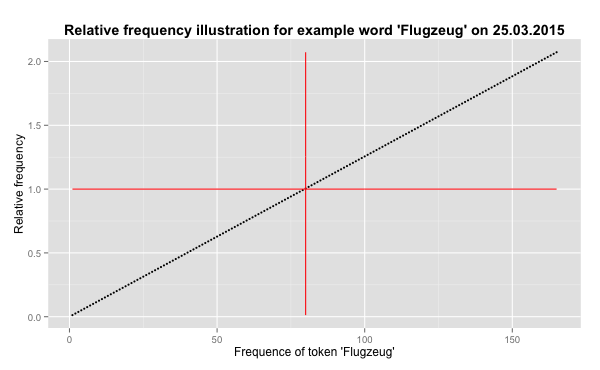
\includegraphics[width=1\textwidth]{pictures/relfreqFlugzeug.png}
    \caption{Illustration der relativen Frequenz des Tokens \enquote{Flugzeug} am 25.03.2015}\label{pic.rel_freq}
\end{figure}



\section{Poisson-Maß}\label{subsec.poisson}
Die Idee dieses Ansatzes ist es ein Maß zu nutzen, das die Wahrscheinlich Ausdrückt die gemessene Anzahl von Tokens eines Wortes an einem Tag zu beobachten. Auch hier wird zur Erstellung des Maßes das Referenzkorpus des letzten Jahres genutzt. Die Annahme dieses Ansatzes ist nun, dass dieser Wahrscheinlichkeit die Poisson-Verteilung zugrunde liegt.\\
Die Formel~\ref{equ.poisson} ist die Poisson-Verteilung nach~\cite[S. 338 ff]{heyer06}.
	\begin{equation}\label{equ.poisson}
	P_\lambda(k) = \frac{\lambda^{k}}{k!}  \cdot e^{-\lambda}
	\end{equation}
	$\lambda$: Welche Frequenz wird erwartet \\
	(relativer Anteil im Referenzkorpus $\cdot$ Umfang des Tageskorpus)\\
	$k$: tatsächliches Auftreten von einem Wort k\\
	$P_\lambda(k)$: Erwartete Wahrscheinlichkeit meine Beobachtung k


In Abbildung~\ref{pic.poisson_algemein} ist exemplarisch die Wahrscheinlichkeit der Beobachtung der Token-Häufigkeit des Wortes Flugzeug abgebildet. Die Annahme besagt nun, dass je kleiner die Wahrscheinlichkeit
ist, desto relevanter erscheint ein Wort.

\begin{figure}[h!]
    \centering
    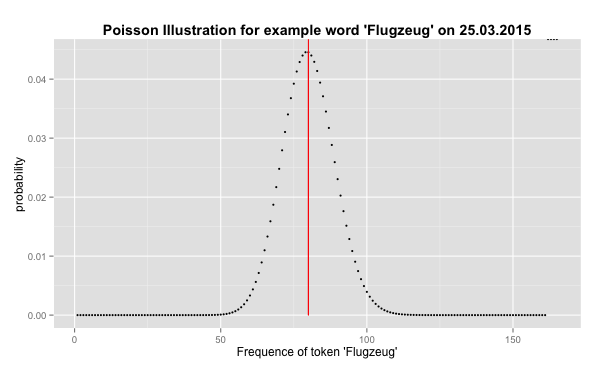
\includegraphics[width=1\textwidth]{pictures/poissonVerteilungFlugzeug.png}
    \caption{Illustration der Poissonverteilung des Token \enquote{Flugzeug} am 25.03.2015}\label{pic.poisson_algemein}
\end{figure}

An der Darstellung wird ein Nachteil dieser Methode deutlich. Nicht nur, wenn ein Token unerwartet oft beobachtet werden kann, auch wenn er seltener als erwartet beobachtet werden kann sinkt die Wahrscheinlichkeit nach diesem Modell beobachtet zu werden und es erscheint als relevantes Wort. Dieses Problem löst die im Folgenden beschriebene Transformation.\\

Ein weiteres Problem stellt der Rechenaufwand für diese Methode dar, da die Fakultät des tatsächlichen Auftretens $k$ eines Wortes berechnet werden muss. Die Herrleitung eines einfacher zu berechnenden 
equivalenten Maßes liefert~\cite[S. 338 ff]{heyer06}. Zu erwähnen ist, dass im Kontext dieser Herleitung das Maß allerdings nicht zur Bestimmung von in dieser Arbeit als relevant angesehenen Einzelwörtern genutzt wird, sondern dient zur Bestimmung signifikanter Kookurenzen. \\
Die Hergeleitete Formel~\ref{equ.poisson_mass} bietet drei Vorteile. Eine Berechnung der Fakultät ist nicht notwendig, die Anwendung des Logarithmus liefert ein positiven Wert für unwahrscheinliche Beobachtungen, wobei die Differenzen gerade bei unwahrscheinlichen Beobachtungen stärker ins Gewicht fallen und zu Letzt werden die Wahrscheinlichkeiten für seltener als erwartet auftretende Worte nicht berücksichtigt. 
 \begin{equation}\label{equ.poisson_mass}
		sig_{poisson}(w) = \frac{k(\log(k)-\log(n\cdot p) -1)}{\log(n)} 
 \end{equation}
k:= Anzahl der Token von w in Tagesbericht\\
n:= Anzahl der Tokens in Tagesbericht\\
p:= relativer Anteil eines Tokens am Jahreskorpus\\

Die Abbildung~\ref{pic.poisson_mass} illustriert die Entwicklung des Poissonmaßes es bezogen auf die Variation des Vorkommens des Tokens Flugzeug. Hier wird sichtbar, dass die unterrepräsentetion keinen positiven Wert erzeugt und somit keinen Einfluss auf eine nach diesem Maß  geordnete Liste hat. In der Praxis sind genügend positive Werte dieses Maß es zu beobachten.\\
Die Formel~\ref{equ.poisson_mass} wurde im praktischen Teil dieser Arbeit genutzt.\\
 
% Hier Beispiel Flugzeug
\begin{figure}[h!]
    \centering
    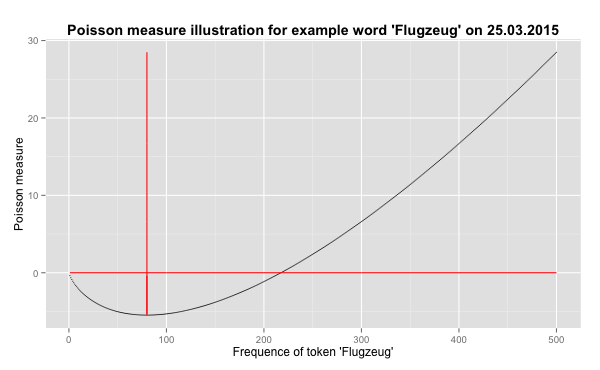
\includegraphics[width=1\textwidth]{pictures/poissonMeasureFlugzeug.png}
    \caption{Illustration des Poisson Maß es des Tokens \enquote{Flugzeug} am 25.03.2015}\label{pic.poisson_mass}
\end{figure}


\subsubsection{Bemerkungen zur Berechnung des Poisson-Maßes}
Die derzeitige Implementierung im Wortschatzporjekt der Universität Leipzig benutzt als Normierungsfaktor nicht die Anzahl aller Tokens im Tagesbericht. Auch zur Bestimmung des relativen Anteils eines Token am Jahreskorpus wird nicht die Anzahl der aller Tokens im Jahreskorpus, sondern die Anzahl der Sätze im Jahreskorpus verwendet. Da bei der verwendeten Zahl von Sätzen das Verhältnis der Anzahl der Wörter zu der Anzahl der Sätze als konstant anzunehmen ist ($\approx 10$), scheint dies gerechtfertigt wie in~\ref{equ.word_sentence} formalisiert. 
\begin{equation}\label{equ.word_sentence}
\frac{|\text{Sätze}_{heute}|}{|\text{Sätze}_{jahr}|} \approx \frac{|Token_{heute}|}{|Token_{Jahr}|}
\end{equation}

Im Abschnitt~\ref{sec.quanitative_auswertung} wird diese Annahme durch einen Vergleich der sich ergebenden relevanten Wörter untersucht.

\section{Termfrequenz inverse Dokumentenfrequenz (tf-idf)}
Die Idee dieses Frequenzmaßes ist es, dass in der natürlichen Sprachverarbeitung breite Anwendung findende Maß TF/IDF für die Aufgabenstellung zu adaptieren. Dabei wird als Dokument das Korpus eines Tages im Referenzzeitraum betrachtet und für jedes Wort im Referenzzeitraum ein Wert bestimmt, der Angibt, an wie vielen Tagen das Wort im Jahr 2014 (Referenzzeitraum) aufgetreten ist. Verlgeiche dazu die Gleichung~\ref{equ.tfidf}.\\
\begin{equation}\label{equ.tfidf}
sig_{tf idf}(w) = \frac{k}{\max(K)} \cdot \log ( \frac{365}{|documentdays(w)|})
\end{equation}
$k$: Frequenz eines Tokens an einem Tag\\
$K$: Alle Frequenzen an einem Tag\\

Als Modifikation wird hier das gängige Verfahren der Logarithmisierung der inversen Dokumentfrequenz angewendet. Des weiteren wird, um eine Vergleichbarkeit über verschiedene Tage hinweg herrstellen zu könnnen, eine Relativierung der Frequenz auf Frequenz des häufigsten Tokens am Tag durchgeführt. Die graue Linie repräsentiert den idf-Wert, der zu der Entsprechung der relativen Tagesfrequenz führt, denn der Logarithmus von 2,7 ist ungefähr 1. Das entspricht dem Auftreten in ca. 8 Tagen des Referenzjahres.\\
% Hier Beispiel Flugzeug
\begin{figure}[h!]
    \centering
    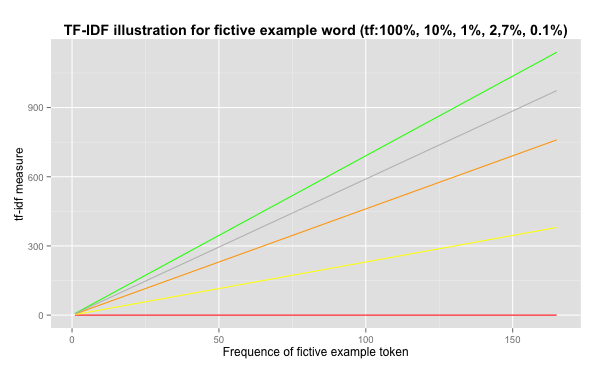
\includegraphics[width=1\textwidth]{pictures/tfidfIllustration.png}
    \caption{Illustration des TF/IDF Maßes anhand eines fiktiven Beispielworts}\label{pic.tfid_mass}
\end{figure}
Die Abbildung~\ref{pic.tfid_mass} verdeutlicht zwei Auswirkungen auf das Finden von relevanten Wörtern für die Aufgabenstellung. Zum einen ist das Grundlegende Problem, welches uns bei dem Maß des relativen Auftretens begegnete, dass niederfrequente Wörter überschätzt werden wieder vorhande, da mit steigender Frequenz die Maßzahl linear wächst. Allerdings wertet die inverse Dokumentenfrequenz häufige Wörter, wie Stoppwörter ab, was hilfreicht erscheint, da diese nicht als interessant zu bewerten sind.
Die rote Linie repräsentiert das Auftreten eines Worten an alle Tagen des Referenzkorpus. Die anderen Geraden bilden eine repräsentative Auswahl an weiteren Anteilen des Wortes an Tagen im Referenzjahr.\\

\section{Termfrequenz inverse Dokumentenfrequenz inverse Quellenfrequenz (tf-idf-isf)}
\emph{Idee: } Wörter sind dann interessant, wenn sie an einem Tag in möglichst vielen verschiedenen Quellen gennant werden.\\
Als Quelle definieren wir die Serveradresse einer Quelle. Diese wird mittels eines regulären Ausdrucks aus den zugeordneten Quellen in der MySQL-Datenbank ermittelt. Als Gesamtzahl der Quellen verwenden wir alle an einem Tag den Wörtern zugeordnete Quellen.\\
Das entstandene Signifikanzmaß wird in Gleichung~\ref{equ.tfidfsf} definiert.
\begin{equation}\label{equ.tfidfsf}
sig_{tf idf isf}(w) = sig_{tf idf}(w) \cdot \log ( \frac{Q_d}{q_d(w)})
\end{equation}
Analog zur inversen Dokumentenfrequenz wird also das tf-idf-Signifikanzmaß mit dem Logarithmus der inversen relativen Anzahl der Quellenfrequenz multipliziert. $Q_d$ ist die Anzahl aller erwähnten Quellen an einem Tag $d$ und $q_d()$ bildet ein Wort auf die Anzahl der Quellen ab, in denen das Wort an Tag $d$  erwähnt wird. 
